% Document class and language
\documentclass{article}
\usepackage{polski}
\usepackage{hyperref}
\usepackage{biblatex}

\addbibresource{literatura.bib}
% Setting geometry
\usepackage[a4paper,top=2cm,bottom=2cm,left=3cm,right=3cm,marginparwidth=1.75cm]{geometry}

% Useful packages
\usepackage{csvsimple}
\usepackage{graphicx}
\usepackage{subcaption}
\usepackage{forest}
\usepackage{listings}
\lstset{language=Python}

\usepackage{xcolor}

\definecolor{codegreen}{rgb}{0,0.6,0}
\definecolor{codegray}{rgb}{0.5,0.5,0.5}
\definecolor{codepurple}{rgb}{0.58,0,0.82}
\definecolor{backcolour}{rgb}{0.95,0.95,0.92}

\lstdefinestyle{pythonstyle}{
    backgroundcolor=\color{backcolour},   
    commentstyle=\color{codegreen},
    keywordstyle=\color{magenta},
    numberstyle=\tiny\color{codegray},
    stringstyle=\color{codepurple},
    basicstyle=\ttfamily\footnotesize,
    breakatwhitespace=false,         
    breaklines=true,                 
    captionpos=b,                    
    keepspaces=true,                 
    numbers=left,                    
    numbersep=5pt,                  
    showspaces=false,                
    showstringspaces=false,
    showtabs=false,                  
    tabsize=2
}

\lstdefinestyle{basicstyle}{
    backgroundcolor=\color{backcolour},   
    basicstyle=\ttfamily\footnotesize,
    breakatwhitespace=false,         
    breaklines=true,                 
    captionpos=b,                    
    keepspaces=true,                 
    numbers=left,                    
    numbersep=5pt,                  
    showspaces=false,                
    showstringspaces=false,
    showtabs=false,                  
    tabsize=2
}

\lstset{style=pythonstyle}

\setcounter{secnumdepth}{3}


\title{Metoda trójwymiarowego modelowania obszarów urbanistycznych z wykorzystaniem metod fotogrametrii}

\author{
    \small Daniel Borkowski\\
    \and
    \small Julia Farganus\\
    \and
    \small Rafał Mielniczuk\\
    \and
    \small Katarzyna Wochal\\
}
\date{12.2024}
\renewcommand\refname{Źródła}

\begin{document}


\begin{titlepage}
    \begin{center}
        \Large
        Politechnika Wrocławska\\
        Wydział Informatyki i Telekomunikacji\\
        \vspace*{1cm}
            
        \Huge
        \textbf{ZESPOŁOWE PRZEDSIĘWZIĘCIE INŻYNIERSKIE}

        \vspace{1.5cm}
        \huge
        \textbf{Metoda trójwymiarowego modelowania obszarów urbanistycznych \\z wykorzystaniem metod fotogrametrii}

        \vspace{1.5cm}
        \LARGE
        Julia Farganus\\
        Katarzyna Wochal\\
        Daniel Borkowski\\
        Rafał Mielniczuk\\

        \vspace{1.5cm}
        Opiekun pracy\\
        dr hab. inż. Marek Krótkiewicz, prof. PWr

        \vfill
            
            
        \vspace{0.8cm}
            
            
        \Large
        Wrocław, 2024
        
            
    \end{center}
\end{titlepage}

\tableofcontents

\section{Wprowadzenie}

Przedmiotem projektu było wykonanie aplikacji wykorzystującej metody fotogrametrii do modelowania trójwymiarowych scen miejskich. Zaimplementowany program umożliwia użytkownikowi zrekonstruowanie chmury punktów i modelu 3D na podstawie podanych na wejściu zdjęć fotogrametrycznych za pomocą dostosowanych do specyfiki problemu w toku eksperymentów rozwiązań \textit{structure from motion} i \textit{gaussian splatting}. Otrzymana w ten sposób chmura może być przez użytkownika poddana segmentacji semantycznej, przeprowadzanej przez wytrenowany do tego celu model sztucznej inteligencji w postaci sieci neuronowej. Aplikacja oferuje również wizualizację wykonanych obliczeń, która możliwa jest dzięki użyciu przystosowanego dla większej wydajności mechanizmu renderowania.

Wytworzony produkt informatyczny ze względu na integrację wielu rozwiązań i efektywną implementację procesu \textit{end-to-end} przejawia potencjał w zastosowaniach biznesowych począwszy od branż takich jak gry wideo, przez architekturę, robotykę, pojazdy autonomiczne, skończywszy na modelowaniu urbanistycznym.

\subsection{Cel i zakres prac}

Rekonstrukcja, klasyfikacja i wizualizacja scen urbanistycznych to dynamicznie rozwijające się zagadnienie, które zyskało na znaczeniu dzięki rosnącej dostępności nowoczesnych technologii, takich jak LiDAR, oraz postępowi w dziedzinie sztucznej inteligencji. Kluczowym wyzwaniem pozostaje jednak efektywne przetwarzanie ogromnych zbiorów danych – chmur punktów, które nierzadko obejmują miliony elementów. Choć na rynku istnieją liczne programy i algorytmy wspierające tego typu analizy, ich skuteczne wykorzystanie w praktyce bywa problematyczne, głównie z uwagi na skalę i złożoność danych urbanistycznych.

Rozwiązanie będzie umożliwiało przeprowadzenie rekonstrukcji do modelu trójwymiarowego na podstawie odpowiednio przygotowanego zbioru zdjęć, klasyfikację otrzymanej sceny na zbiór pre-definiowanych klas istotnych w kontekście urbanistycznym, oraz wizualizację wykonanych obliczeń. 

Poniżej znajdują się cele, które zostaną zrealizowane w przedsięwzięciu:

\begin{enumerate}
    \item skomponowanie własnego zbioru danych, 
    \item wykorzystanie algorytmu Gaussian Splatting do rekonstrukcji sceny 3D,
    \item filtracja chmury punktów przy użyciu różnych technik, 
    \item zastosowanie architektur sieci neuronowych takich jak PointNet do klasyfikacji chmury punktów, 
    \item adaptacja istniejących bibliotek do wizualizacji wyników, 
    \item implementacja własnego algotymu do renderowania gaussianów.
\end{enumerate}

\section{Stan wiedzy w obszarze przedsięwzięcia}



\subsection{Rekonstrukcja}

Wirtualne reprezentacje krajobrazów miejskich są coraz bardziej wykorzystywane w różnego rodzaju zadaniach. Mimo rozwoju technik, począwszy od pozyskiwania danych (np. LiDAR), skończywszy na parametrycznych modelach (np. sieci neuronowe), zadanie modelowania pozostawia nierozwiązane problemy wpływające na jakość modelu wynikające z np. trudności akwizycji danych. 
Istnieje wiele sposobów rekonstrukcji które można podzielić ze względu na dane wejściowe, poziom szczegółowości, automatyzację czy też dane wyjściowe. W naszym projekcie rekonstrukcja zachodzi na dwóch etapach - najpierw jako chmura punktów, następnie jako zbiór splatów. 

\subsubsection{Structure from motion}
Structure from motion (SfM)\cite{Schonberger_2016_CVPR} to technika fotogrametryczna służąca do szacowania struktur trójwymiarowych na podstawie zbiorów dwuwymiarowych obrazów, opierająca się na odnajdywaniu wspólnych punktów między obrazami. Jednym z wyróżnianych podejść jest inkrementalne SfM\ref{fig:sfm_flow}, zawierające komponent iteracyjnej rekonstrukcji. Proces składa się z kilku kluczowych etapów:
\begin{enumerate}
  \item Ekstrakcja cech - przy wykorzystaniu algorytmów takich jak SIFT czy jego pochodne, zapewniających odporność na zmiany rotacji bądź oświetlenia, na każdym z obrazów wykrywane są punkty charakterystyczne, reprezentowane matematycznie przy pomocy deskryptorów;
  \item Dopasowywanie cech - pary obrazów testowane są pod kątem nakładania się sceny; punkty charakterystyczne z jednego obrazu są dopasowywane do odpowiadających im punktów na innych obrazach na podstawie podobieństwa deskryptorów;
  \item Weryfikacja geometryczna - SfM weryfikuje poprawność dopasowań cech, próbując oszacować transformację mapującą punkty między obrazami za pomocą geometrii rzutowej. Jeżeli transformacja odwzorowuje wystarczającą liczbę punktów, dopasowanie jest uznawane za zweryfikowane;
  \item Kroki rekonstrukcji inkrementalnej:
    \begin{itemize}
      \item \textbf{inicjalizacja} modelu oparta na wyborze pary obrazów o dużym pokryciu cech wspólnych,
      \item \textbf{rejestracja} kolejnych obrazów w modelu z wykorzystaniem dopasowań do punktów z już dodanych do niego obrazów, obejmująca szacowanie pozycji kamer,
      \item \textbf{triangulacja} nowych punktów występujących na przynajmniej dwóch obrazach zwiększająca pokrycie sceny i stabilność modelu,
      \item \textbf{regulacja wiązki} (\textit{ang. bundle adjustment}), czyli optymalizacja parametrów kamer i parametrów punktów minimalizująca błędy reprojekcji,
      \item \textbf{usuwanie punktów odstających}.
    \end{itemize}
\end{enumerate}
Głównymi wynikami procesu jest przeważnie zestaw wyznaczonych punktów 3D oraz obliczone pozycje i orientacje kamer.

\begin{figure}[!ht]
  \includegraphics[width=\linewidth]{img/sfm_pipeline.png}
  \caption{Przepływ inkrementalnego SfM}
  \label{fig:sfm_flow}
\end{figure}

\subsubsection{Gaussian Splatting}

Popularną techniką rekonstrukcji z chmury punktów jest siatka (ang. mesh), wykorzystana np. w pracy City3D\cite{city3D}. Często jednak uzyskanie dobrej jakości siatki wymaga kombinacji wielu różnych geometrycznych algorytmów. Wraz z rozwojem sztucznej inteligencji zaczęły pojawiać się i w dziedzinie rekonstrukcji rozwiązania wykorzystujące sieci neuronowe - takie jak np. NeRF\cite{nerf}, gdzie informacje o scenie zawarte są w wagach modelu. Niedoskonałością tego rozwiązania jest jednak długi czas trenowania nawet dla sceny jednego obiektu, wahający się od parunastu godzin do paru dni. Z pomocą przychodzą inne metody, jak np. Gaussian Splatting \cite{gaussiansplatting}, który rezygnuje w całości z sieci neuronowej i wykorzystuje zbiór tzw. "splatów" do zbudowania sceny. Jako że w naszym projekcie stawiamy na optymalne wykorzystanie zasobów, to zdecydowaliśmy się na wybór właśnie ostatniej z wymienionych metod. 

\begin{figure}[!htb]
    % images need to be the same size
    \minipage{0.32\textwidth}
      \includegraphics[width=\linewidth]{img/sota/city3dmesh.jpg}
      \caption{City3D - siatka}\label{fig:mesh_example}
    \endminipage\hfill
    \minipage{0.32\textwidth}
      \includegraphics[width=\linewidth]{img/sota/nerfobject.jpg}
      \caption{Nerf - sieć neuronowa}\label{fig:nerf_example}
    \endminipage\hfill
    \minipage{0.32\textwidth}%
      \includegraphics[width=\linewidth]{img/sota/gaussiansplattingobject.jpg}
      \caption{Gaussian Splatting - splat'y}\label{fig:gaussplat_example}
    \endminipage
\end{figure}

Splat (tłum. punkt rozmyty) jest rozszerzeniem punktu i posiada atrybuty
\begin{itemize}
    \item środek (x, y, z)
    \item kolor
    \item przeźroczystość
    \item macierz kowariancji (koduje rotację i skalę)
\end{itemize}

Najlepszy zbiór splatów opisujący scenę jest znajdowany w procesie optymalizacji opisanym poniżej schematem

\begin{figure}[!htb]
    \includegraphics[width=\linewidth]{img/sota/gaussian_splatting_flow.png}
    \caption{Optymalizacja zbioru splatów}\label{fig:splatting_algorithm}
\end{figure}

\begin{enumerate}
    \item Wykorzystanie chmury punktów z rekonstrukcji do inicjalizacji zbioru splatów
    \item Rzutowanie perspektywiczne 3-wymiarowych gaussianów na obraz widziany z danej kamery, czego wynikiem jest zbiór dysków
    \item Renderowanie polegające na akumulowaniu dla każdego piksela wkładu od różnych nachodzących dysków 
    \item Obliczanie funkcji straty - porównanie z prawdziwym obrazkiem z danej kamery
    \item Adaptacja gęstości gaussianów - klonowanie, dzielenie lub usuwanie wg. kryteriów zależnych od strategii
\end{enumerate}

Niestety metoda ta nie pozostaje bez wad. W przypadku dużych zbiorów danych zużycie pamięci może wynieść nawet parę GB, co wymaga dobrej jakości karty graficznej. Inną kwestią jest duża liczba hiperparametrów, które często wymagają ręcznego dostosowania do danej sceny. 

\subsection{Segmentacja}
Warto nadmienić, że nie jest to segmentacja \cite{pointnet}.

\section{Projekt}

\subsection{Specyfikacja wymagań na produkt programowy}

\begin{figure}[!htb]
    \includegraphics[width=1.0\linewidth]{img/diagramy/zpi use case.png}
    \caption{Diagram przypadków użycia}\label{fig:use_case_diagram}
  \end{figure}

\subsection{Architektura}

\begin{figure}[!htb]
    \includegraphics[width=1.0\linewidth]{img/diagramy/diagram_wdrozenia_komponentow_3.png}
    \caption{Diagram wdrożenia komponentów}\label{fig:components_diagram}
\end{figure}


\subsection{Implementacja}

\subsection{Technologie}

W projekcie wykorzystano następujące technologie

\begin{itemize}
    \item \textbf{C/C++}: OpenCL, OpenGL
    \item \textbf{Python}: Pytorch, pycolmap, open3d, pyvista, PyQt (numpy, matplotlib), pytest
    \item CloudCompare, Meshlab
    \item \textbf{GPU}
    \item Jira, Confluence, Github, Discord
\end{itemize}

\begin{figure}[!ht]
    \centering
    \includegraphics[width=0.9\linewidth]{img/sota/technologie.png}
  \end{figure}

\subsubsection{Struktura plikowa projektu}

% millon opcji https://tex.stackexchange.com/questions/5073/making-a-simple-directory-tree
\begin{forest}
  for tree={
    grow'=0,
    child anchor=west,
    parent anchor=south,
    anchor=west,
    calign=first,
    edge path={
      \noexpand\path [draw, \forestoption{edge}] (!u.south west) ++(3pt,0) -- +(-3pt,0) |- (.child anchor)\forestoption{edge label};
    },
    before typesetting nodes={
      if n=1
        {insert before={[,phantom]}}
        {}
    },
    fit=band,
    before computing xy={l=15pt},
  }
[project
  [data
    [city\_model
      [images]
      [sparse
          [images.bin]
          [cameras.bin]
          [points.bin]
          [sparse.ply]
      ]
      [filtered\_model.ply]
      [model.pt]
      [model.ply]
      [model\_seg.ply]
    ]
    [pointnet-ckpt.pt]
  ]
  [scripts]
  [src
    [frontend]
    [backend]
    [urb3d
      [datasets]
      [pipeline]
      [segmentation]
      [rendering]
      [geometry]
      [models]
      [splats]
    ]
  ]
  [test]
]
\end{forest}

\subsection{Gaussian Splatting}
Przy pomocy biblioteki \textit{gsplat}\cite{ye2024gsplatopensourcelibrarygaussian} zawierającej implementację \textit{Gaussian Splatting} w Pythonie wykonaliśmy eksperymenty polegające na uruchomeniu algorytmu dla różnych wartości hiperparametrów w celu znalezienia wartości, które prowadzą do jak najbardziej optymalnego procesu trenowania w kontekście czasu trwania i wykorzystania pamięci. 

Na wejściu algorytmu podawana jest otrzymywana w procesie rekonstrukcji chmura punktów, która jest bazą do dalszego dzielenia i powstawania "gaussianów", a ich parametry: pozycja, kolor, skala i rotacja są optymalizowane przy pomocy metody spadku wzdłuż gradientu. Metryki przyjęte do oceny jakości to SSIM (Structural Similarity Index Measure), PSNR (Peak Signal-to-Noise Ratio) oraz LPIPS (Learned Perceptual Image Patch Similarity).

W wyniku przeprowadzenia eksperymentów okazało się, że najważniejszymi sterującymi procesem parametrami są 
\begin{enumerate}
    \item Liczba Gaussianów: w przypadku scen urbanistycznych w celu oddania odpowieniej szczegółowości potrzebne jest parę milionów Gaussianów, dla naszych scen było to zwykle 3 mln.
    \item Strategia i częstość adaptacji: określają w jaki sposób oraz jak często dodawane i usuwane są Gaussiany. 
    \item Liczba iteracji: zwykle im dłużej trenowana jest scena tym lepsze wyniki otrzymujemy, jednak zależy to również od przyjętej strategii. Liczba ta wpływa bezpośrednio na czas trenowania, powinna wynieść nie mniej niż paręnaście tysięcy.
    \item Stopień zmiennych harmonicznych: wyrażają one kolor, im większy stopień tym lepsza jakość sceny, ale też zwiększone zużycie pamięci.  
\end{enumerate}

Poniżej przedstawione są przykładowe wizualizacje. Renderowania zostały wykonane przy pomocy biblioteki nerfview która również służy do wizualizacji splatów. Na poniższych rysunkach są od lewej do prawej: prawdziwe zdjęcie i widok modelu.

\begin{figure}[!h]
    \centering
    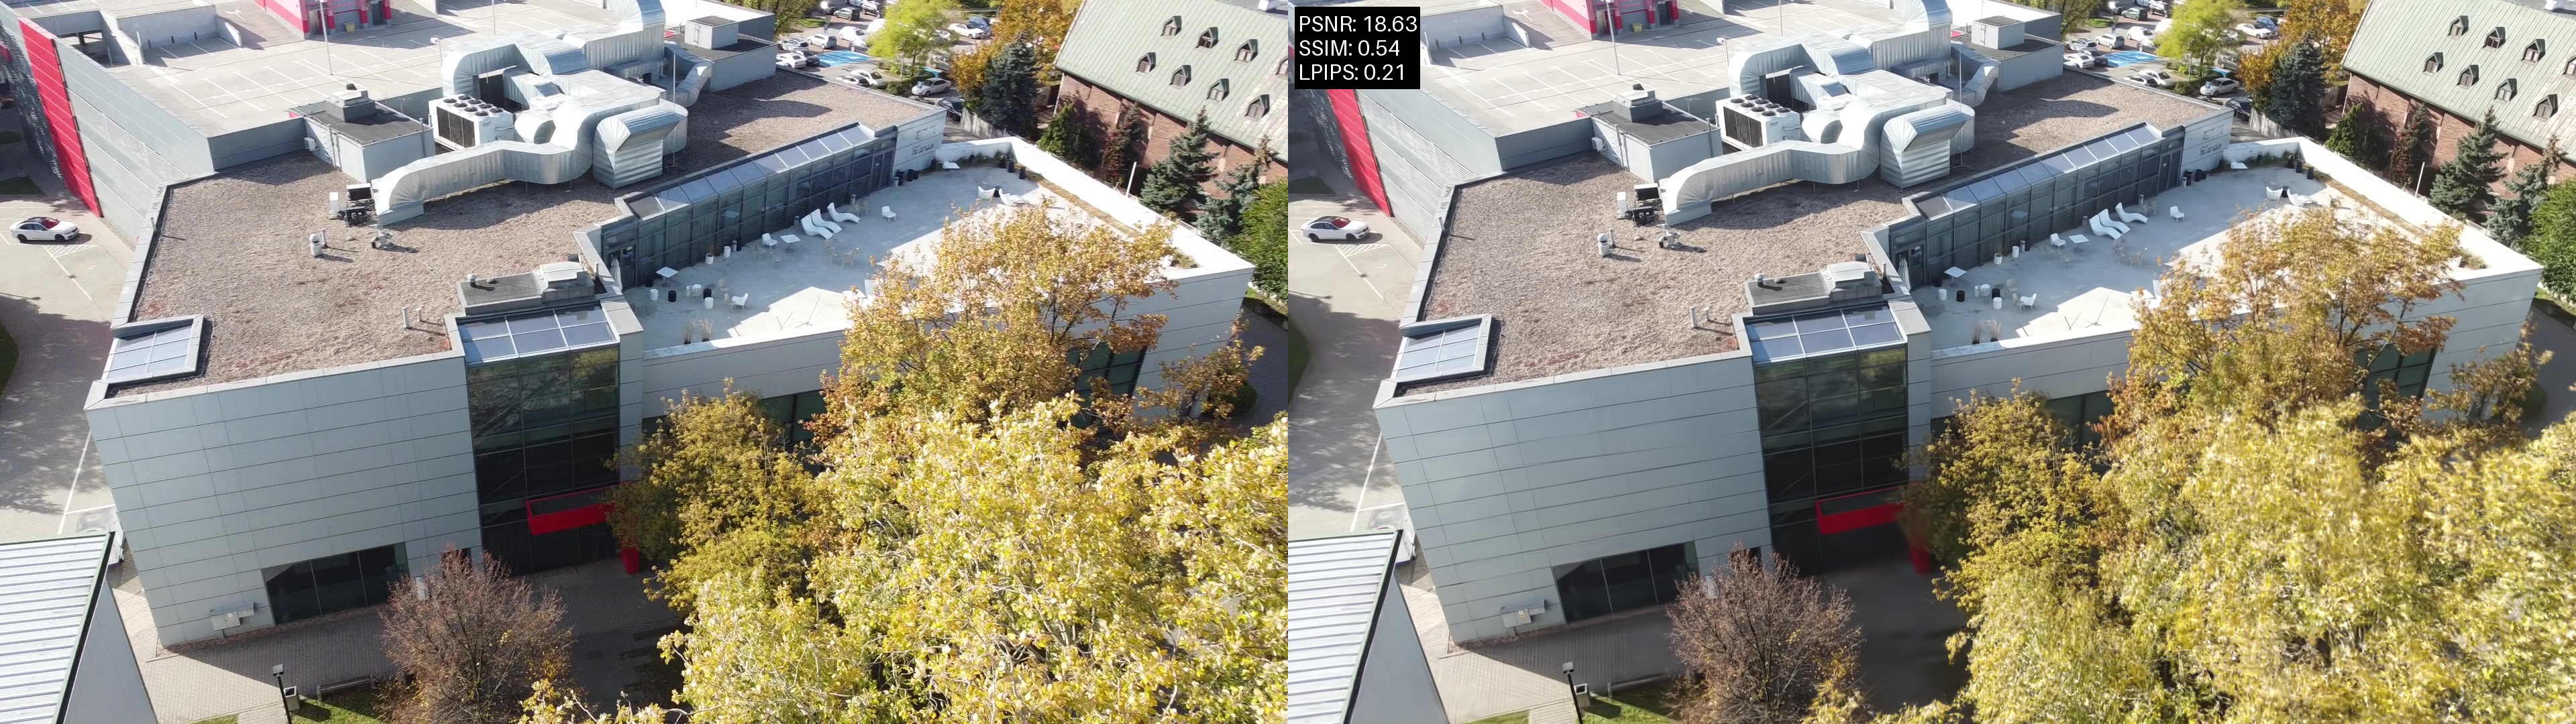
\includegraphics[width=1.0\linewidth]{images/sks_viper_0008.png}
    \caption{Scena SKS}
    \label{fig:sks_gs}
\end{figure}

\begin{figure}[!h]
    \centering
    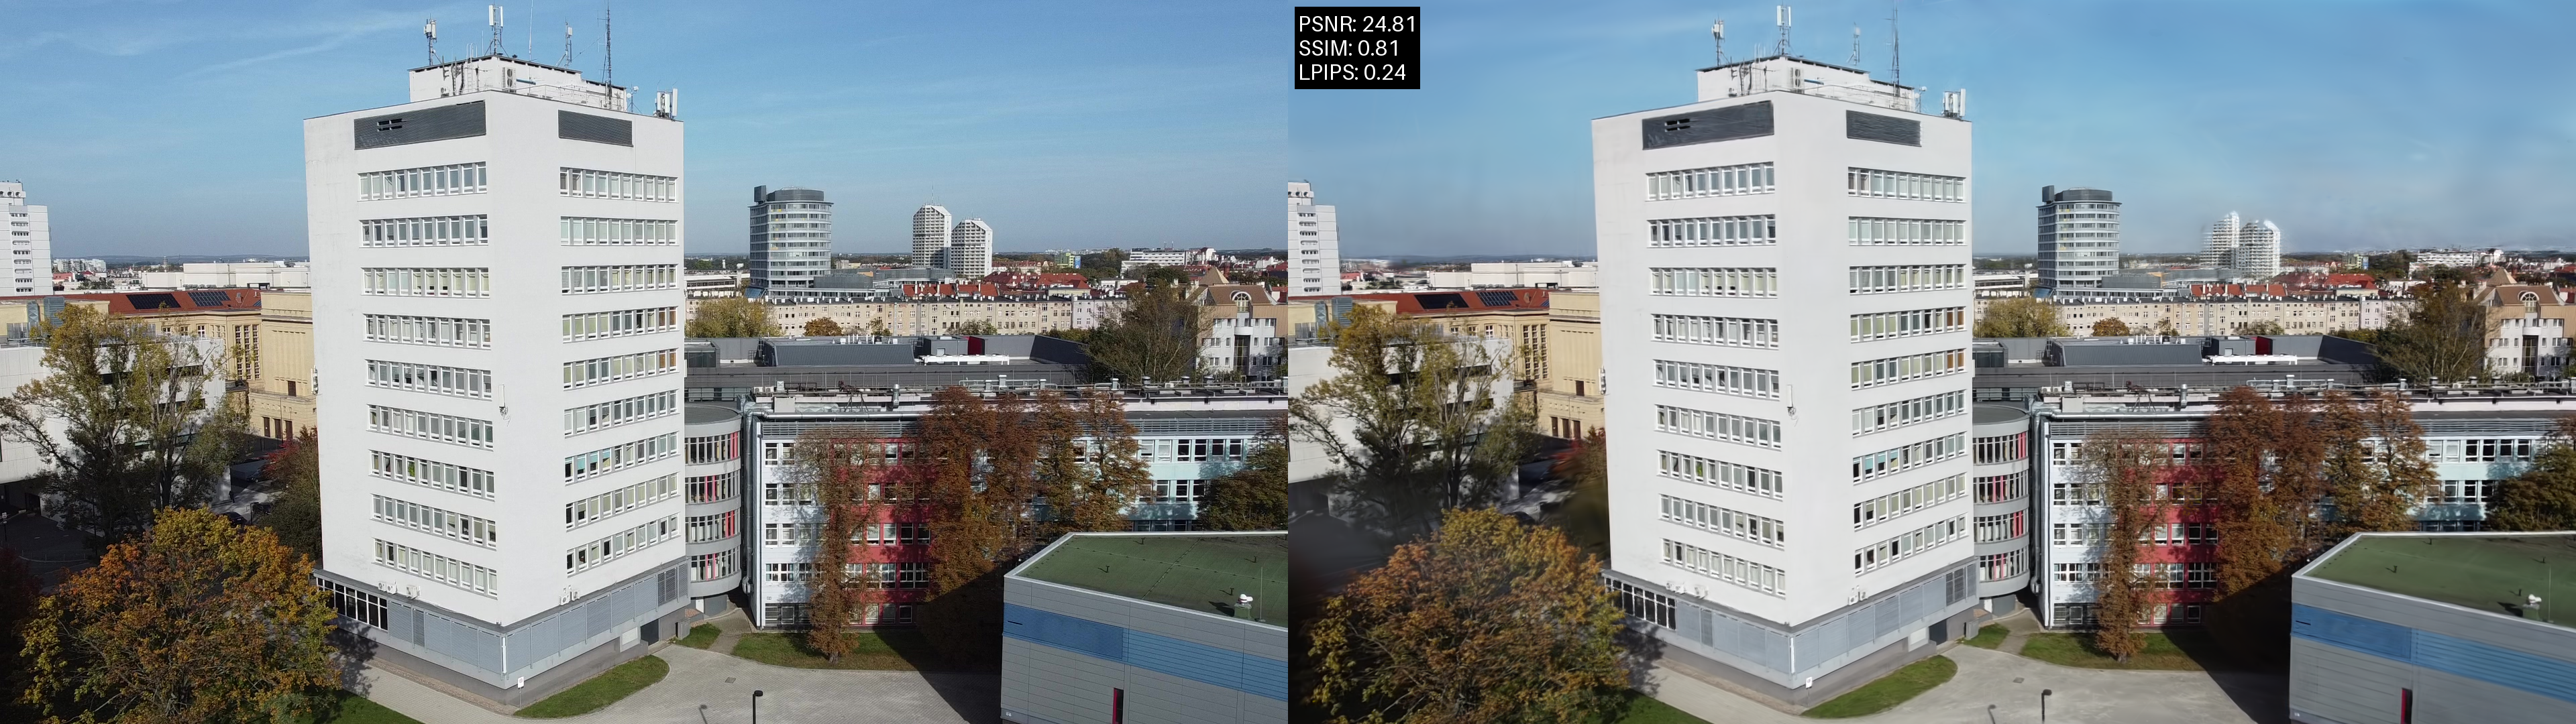
\includegraphics[width=1.0\linewidth]{images/c5_mouse_0001.png}
    \caption{Scena C5}
    \label{fig:c5_gs}
\end{figure}

\begin{figure}[!h]
    \centering
    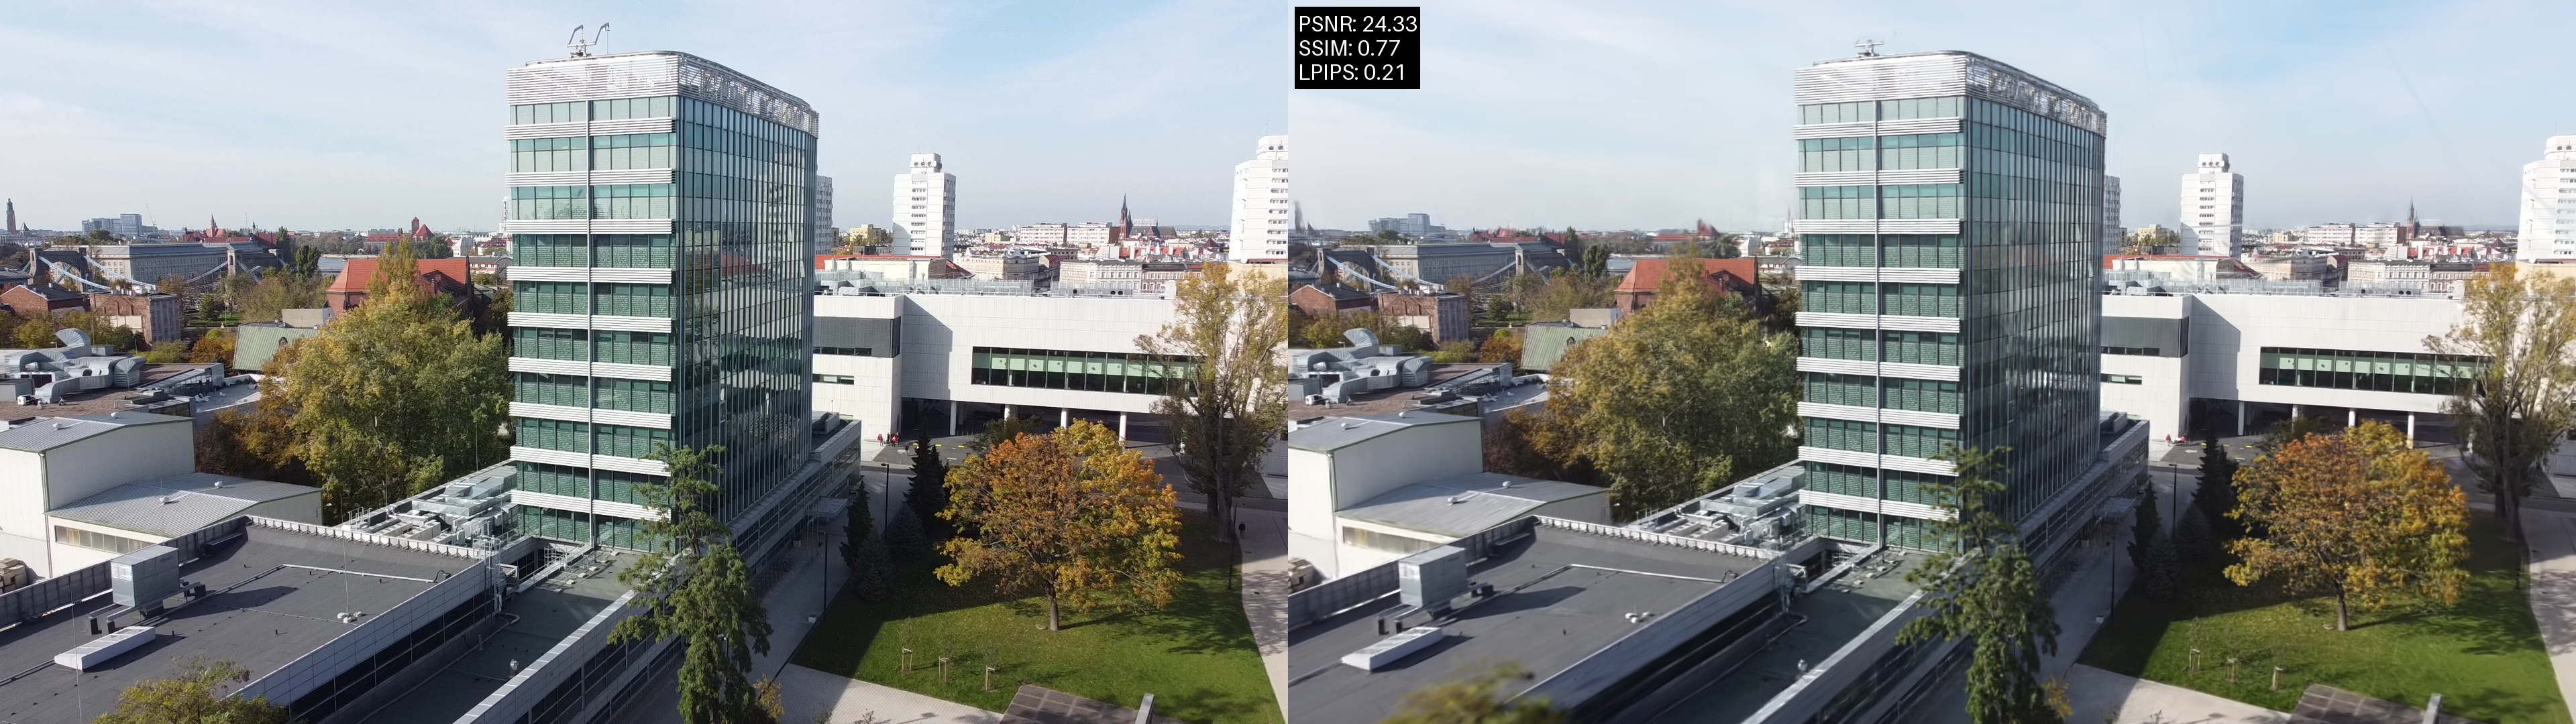
\includegraphics[width=1.0\linewidth]{images/c7_gepard_0006.png}
    \caption{Scena C7}
    \label{fig:c7_gs}
\end{figure}

\subsection{Testy}

W ramach przetestowania poprawności kodu zostały wykonane dla części skryptów testy jednostkowe przy pomocy biblioteki \textit{pytest}.

\lstset{style=basicstyle}
\begin{lstlisting}
scripts\test_colmap_reconstruction.py::test_colmap_reconstruction_files_exist 
scripts\test_distance_pcd_filtering.py::test_distance_pcd_filtering_files_exist 
scripts\test_distance_pcd_filtering.py::test_distance_pcd_filtering_works 
scripts\test_distance_pcd_filtering.py::test_error_on_wrong_type 
scripts\test_save_model.py::test_save_model 
scripts\test_save_model.py::test_fail_on_wrong_path_name 
scripts\test_segmentation.py::test_segmentation_files_exist 
scripts\test_segmentation.py::test_segmentation_class_is_added 
scripts\test_segmentation.py::test_segmentation_classes_are_in_range 
scripts\test_segmentation.py::test_segmentation_fails_on_corrupted_input 
scripts\test_simple_trainer.py::test_simple_trainer_files_exist 
scripts\test_simple_trainer.py::test_simple_trainer_pt_file_is_correct 
scripts\test_simple_trainer.py::test_training_fails_on_incomplete_input 
scripts\test_statistical_pcd_filtering.py::test_error_on_wrong_type 
\end{lstlisting}

Testy obejmowały m. in. sprawdzenie poprawności powstałych plików oraz występowania błędów. 


\section{Wyniki}

\subsection{Funkcjonalność oprogramowania}

Modularność naszego projektu sprawia, że wygodniej jest omówić niezależnie każdą z części. Dla jasności, przebieg całego procesu jest następujący:
\begin{enumerate}
    \item Wczytanie plików zdjęć.
    \item Rekonstrukcja SFM do chmury punktów, która jest podstawą do kolejnego etapu.
    \item Wytrenowanie modelu sceny przy pomocy algorytmu Gaussian Splatting.
    \item Filtracja, następnie segmentacja chmury punktów z poprzedniego kroku.
\end{enumerate}
Każda funkcjonalność, jak i wizualizacje wyników poszczególnych zadań są dostępne poprzez interfejs użytkownika. 

\subsection{Akwizycja danych}
W projekcie założono wykorzystanie metod fotogrametrycznych do tworzenia trójwymiarowych modeli obszarów urbanistycznych. Za część projektu przyjęto z tego względu również pozyskanie własnych
zestawów danych fotograficznych (fotogramów), które spełniałyby wymogi techniczne, umożliwiające
późniejszą rekonstrukcję 3D. Wynikowe zbiory zdjęć powstały poprzez wykonanie dużej liczby ujęć, obejmujących wiele kątów i perspektyw oraz zapewniając odpowiednie nakładanie się obrazów dla poprawnego działania oprogramowania fotogrametrycznego.


Akwizycję zrealizowano na kampusie Politechniki Wrocławskiej, koncentrując się na budynkach C5,
C7 oraz Strefie Kultury Studenckiej (SKS)[\ref{fig:four-photos}] i pozyskując zdjęcia zarówno z lotów bezzałogowym statkiem powietrznym, jak i z poziomu gruntu. W jej wyniku przygotowano własne kompletne zbiory danych, które spełniły wymogi jakościowe i posłużyły do budowy testowych modeli.

\begin{figure}[h!]
    \centering
    \begin{minipage}{0.24\textwidth}
        \centering
        \includegraphics[width=\textwidth]{img/sks_dataset_1.jpg}
    \end{minipage}
    \hfill
    \begin{minipage}{0.24\textwidth}
        \centering
        \includegraphics[width=\textwidth]{img/sks_dataset_2.jpg}
    \end{minipage}
    \hfill
    \begin{minipage}{0.24\textwidth}
        \centering
        \includegraphics[width=\textwidth]{img/sks_dataset_3.jpg}
    \end{minipage}
    \hfill
    \begin{minipage}{0.24\textwidth}
        \centering
        \includegraphics[width=\textwidth]{img/sks_dataset_4.jpg}
    \end{minipage}
    \caption{Przykładowe zdjęcia z akwizycji danych przedstawiające SKS}
    \label{fig:four-photos}
\end{figure}

\subsubsection{Structure from motion}
Jedną z funkcjonalności oferowanych przez przygotowane oprogramowanie jest wyznaczanie struktury przestrzennej sceny w postaci chmury punktów na podstawie zbioru fotogramów przy pomocy techniki Structure from motion. Zaproponowana implementacja opiera się na wykorzystaniu popularnego narzędzia COLMAP\cite{schoenberger2016mvs}\cite{Schonberger_2016_CVPR}, które zostało włączone do projektu w postaci pythonowej biblioteki \href{https://github.com/colmap/pycolmap}{\textit{pycolmap}}. Biblioteka ta oferuje szereg funkcji umożliwiających przeprowadzenie kluczowych etapów procesu SfM, w tym wykorzystane w projekcie funkcjonalności do wykrywania cech charakterystycznych na obrazach, dopasowywania punktów wspólnych między obrazami czy przeprowadzania inkrementalnej rekonstrukcji, która dodatkowo została skonfigurowana za pomocą parametrów dobranych tak, aby zapewnić zadowalającą jakość wyniku przy zachowaniu wydajności.

W wyniku działania tak zaimplementowanego procesu powstają pliki binarne zapisujące dane przede wszystkim wyznaczonych punktów 3D i pozycji kamer. Biblioteka \textit{pycolmap} umożliwiła dodatkowo łatwe wprowadzenie funkcjonalności eksportu wyników do formatu PLY, którego to formatu plik zostaje wykorzystany do wizualizacji wygenerowanej chmury punktów. Z kolei reprezentacja w postaci plików binarnych zostaje w kolejnych etapach wczytywana i po przefiltrowaniu służy za podstawę do modelowania z zastosowaniem algorytmu Gaussian Splatting.

\begin{figure}[!ht]
  \centering
  \includegraphics[width=0.9\linewidth]{img/sfm_projection.png}
  \caption{Projekcja przykładowej chmury punktów na płaszczyznę porównana do zdjęcia}
\end{figure}

\subsection{Gaussian Splatting}
Przy pomocy biblioteki \textit{gsplat}\cite{ye2024gsplatopensourcelibrarygaussian} zawierającej implementację \textit{Gaussian Splatting} w Pythonie wykonaliśmy eksperymenty polegające na uruchomeniu algorytmu dla różnych wartości hiperparametrów w celu znalezienia wartości, które prowadzą do jak najbardziej optymalnego procesu trenowania w kontekście czasu trwania i wykorzystania pamięci. 

Na wejściu algorytmu podawana jest otrzymywana w procesie rekonstrukcji chmura punktów, która jest bazą do dalszego dzielenia i powstawania "gaussianów", a ich parametry: pozycja, kolor, skala i rotacja są optymalizowane przy pomocy metody spadku wzdłuż gradientu. Metryki przyjęte do oceny jakości to SSIM (Structural Similarity Index Measure), PSNR (Peak Signal-to-Noise Ratio) oraz LPIPS (Learned Perceptual Image Patch Similarity).

W wyniku przeprowadzenia eksperymentów okazało się, że najważniejszymi sterującymi procesem parametrami są 
\begin{enumerate}
    \item Liczba Gaussianów: w przypadku scen urbanistycznych w celu oddania odpowieniej szczegółowości potrzebne jest parę milionów Gaussianów, dla naszych scen było to zwykle 3 mln.
    \item Strategia i częstość adaptacji: określają w jaki sposób oraz jak często dodawane i usuwane są Gaussiany. 
    \item Liczba iteracji: zwykle im dłużej trenowana jest scena tym lepsze wyniki otrzymujemy, jednak zależy to również od przyjętej strategii. Liczba ta wpływa bezpośrednio na czas trenowania, powinna wynieść nie mniej niż paręnaście tysięcy.
    \item Stopień zmiennych harmonicznych: wyrażają one kolor, im większy stopień tym lepsza jakość sceny, ale też zwiększone zużycie pamięci.  
\end{enumerate}

Poniżej przedstawione są przykładowe wizualizacje. Renderowania zostały wykonane przy pomocy biblioteki nerfview która również służy do wizualizacji splatów. Na poniższych rysunkach są od lewej do prawej: prawdziwe zdjęcie i widok modelu.

\begin{figure}[!h]
    \centering
    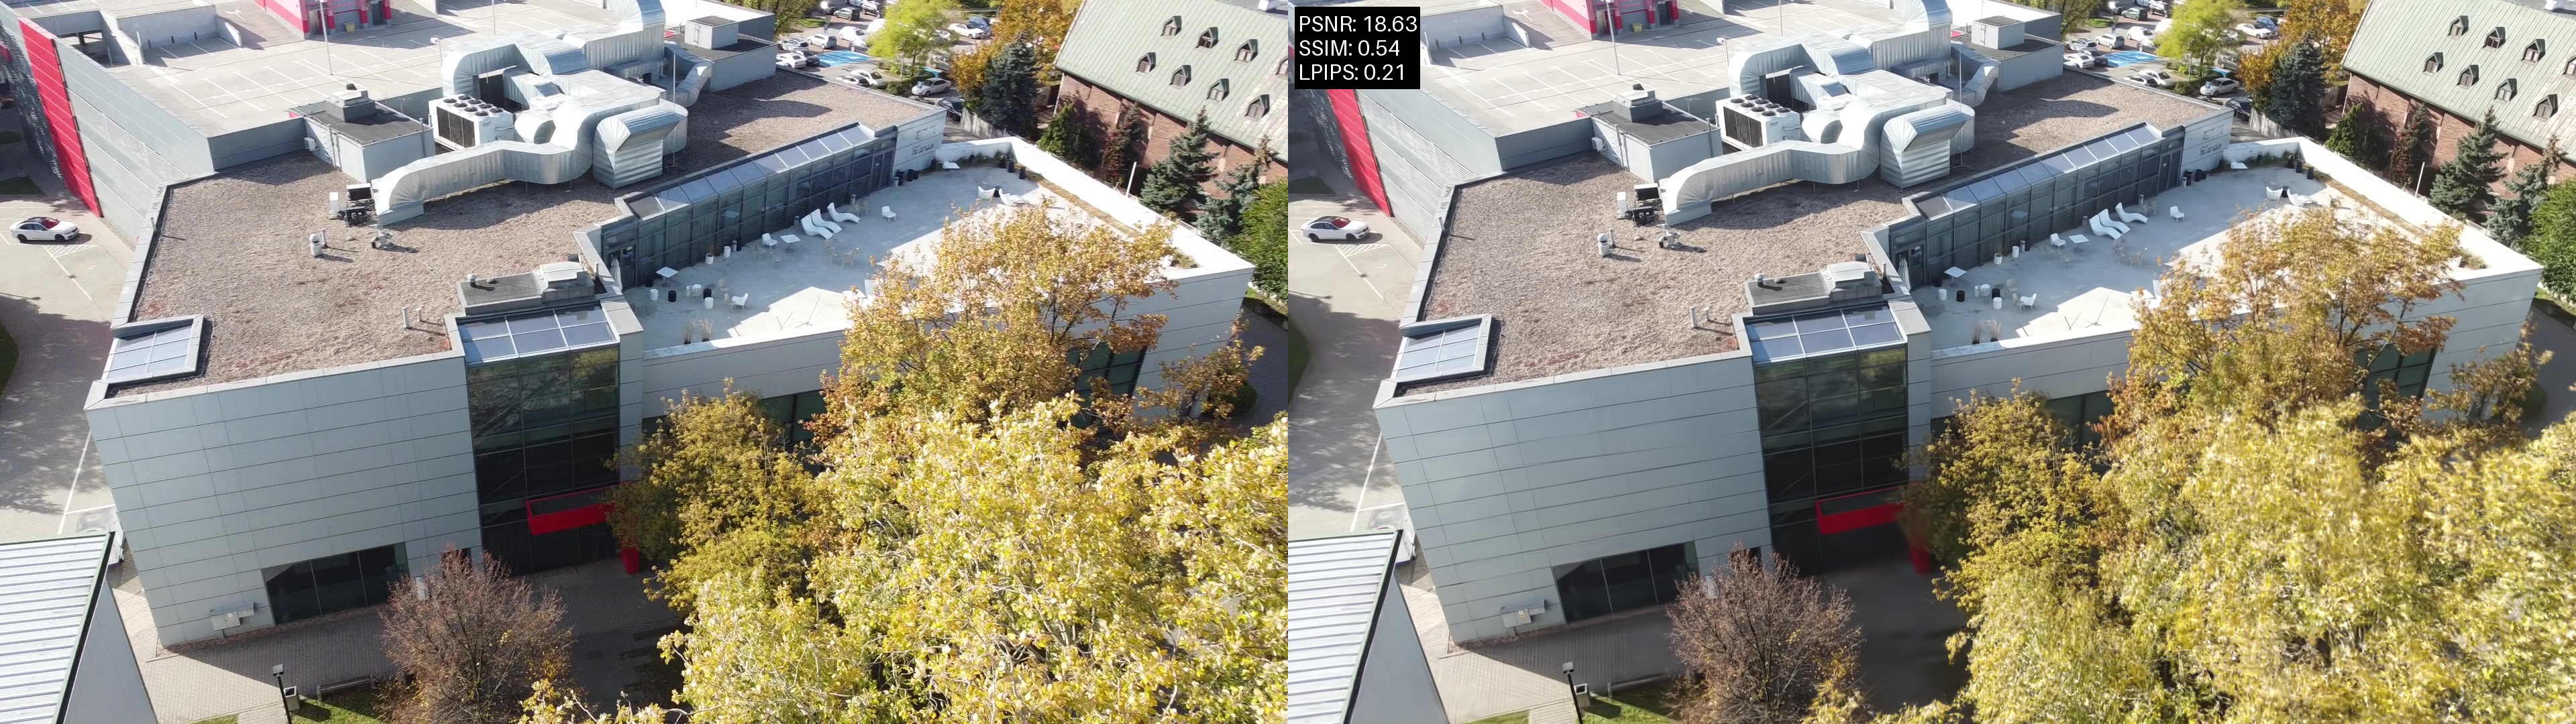
\includegraphics[width=1.0\linewidth]{images/sks_viper_0008.png}
    \caption{Scena SKS}
    \label{fig:sks_gs}
\end{figure}

\begin{figure}[!h]
    \centering
    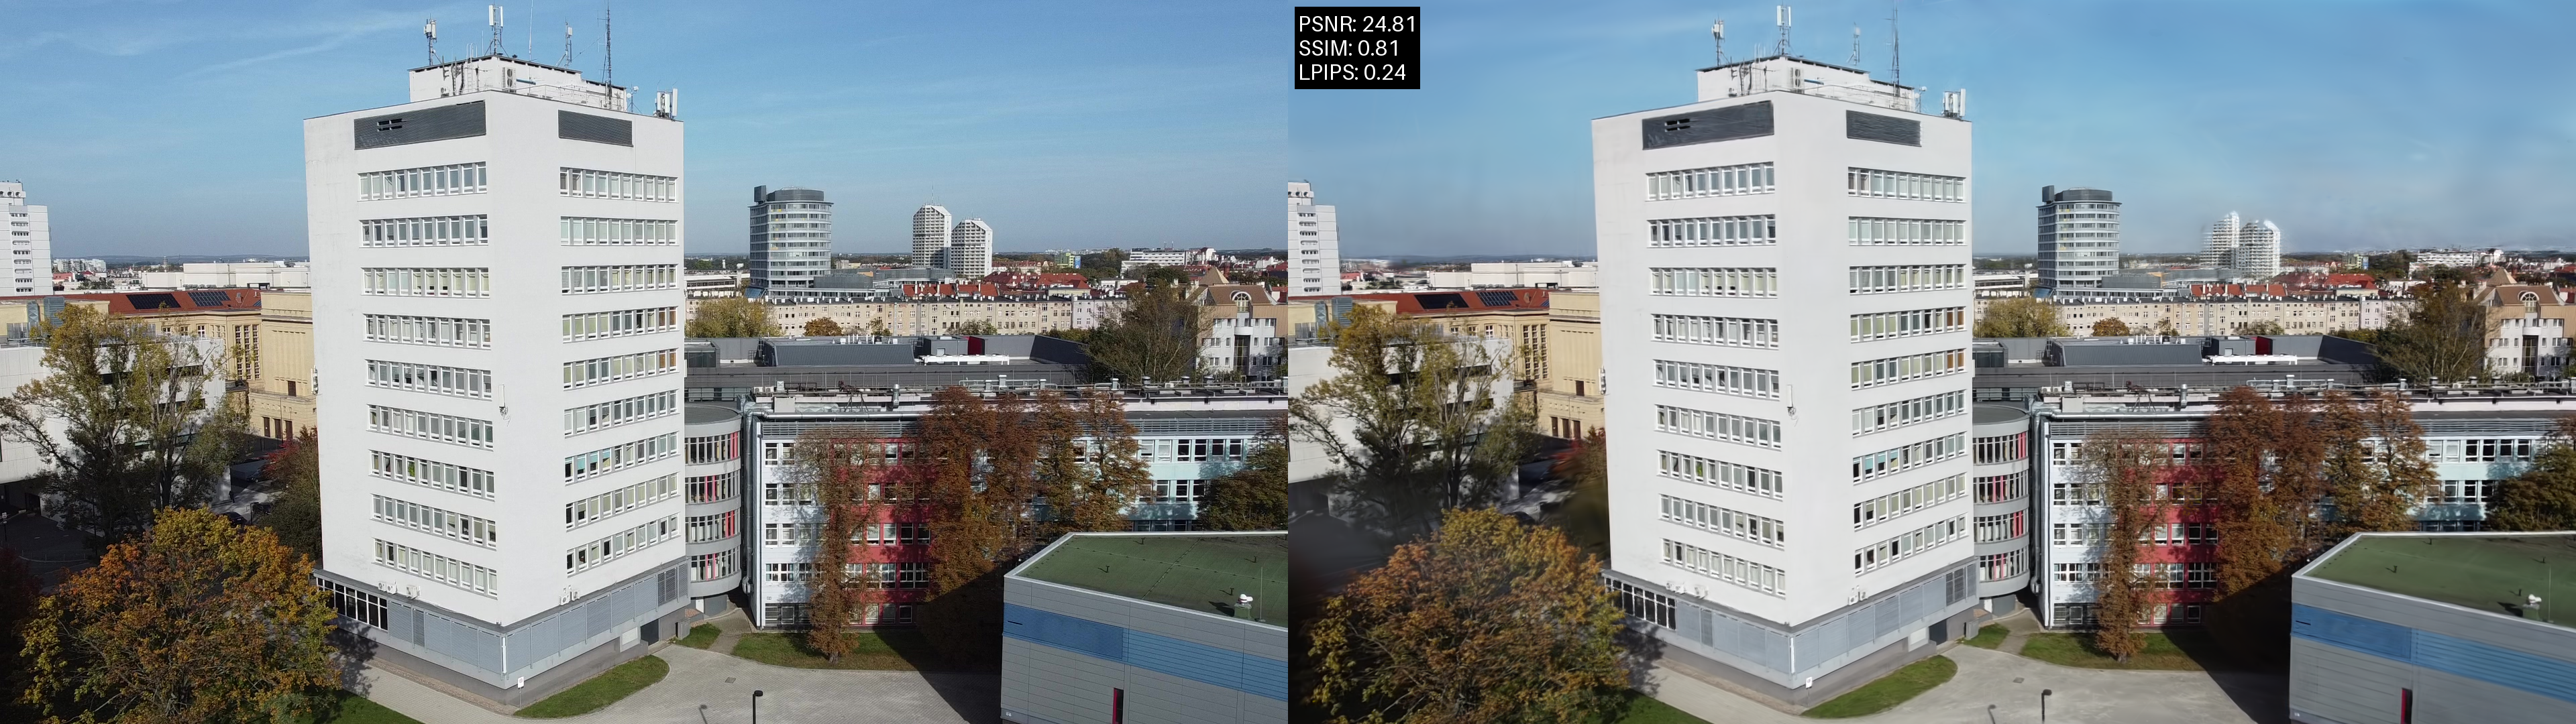
\includegraphics[width=1.0\linewidth]{images/c5_mouse_0001.png}
    \caption{Scena C5}
    \label{fig:c5_gs}
\end{figure}

\begin{figure}[!h]
    \centering
    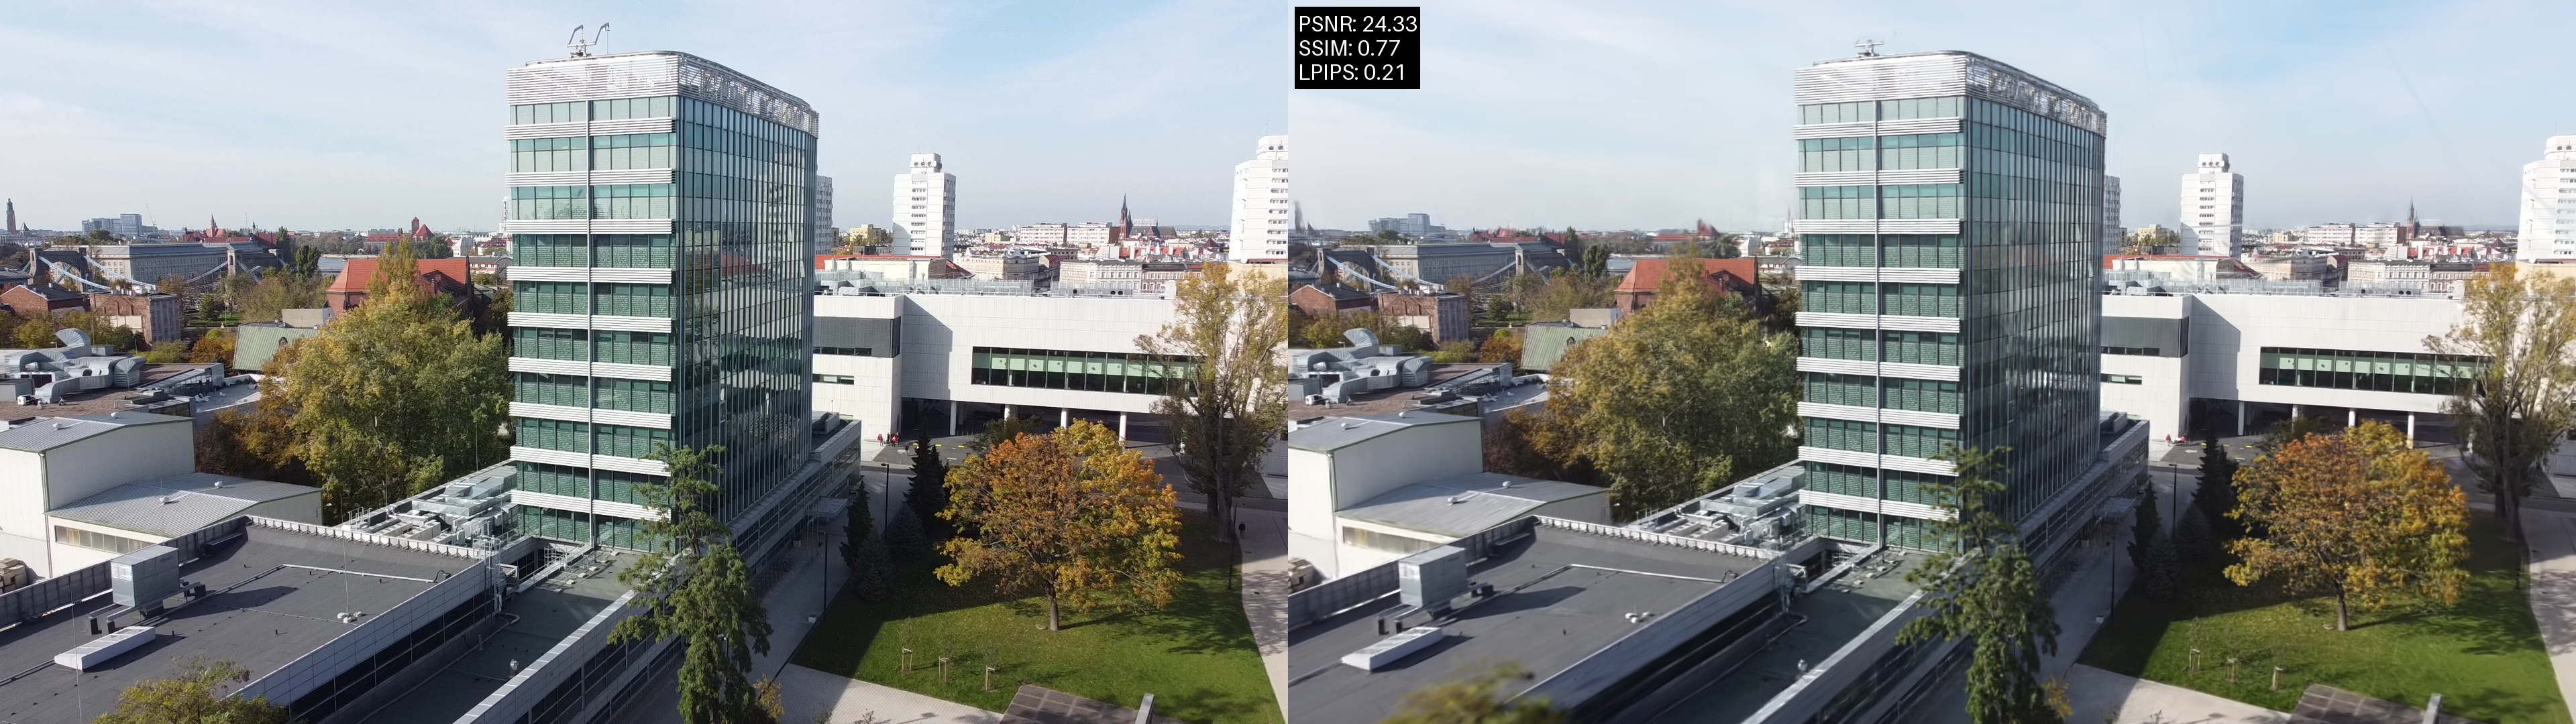
\includegraphics[width=1.0\linewidth]{images/c7_gepard_0006.png}
    \caption{Scena C7}
    \label{fig:c7_gs}
\end{figure}

\subsection{Segmentacja}
Używając biblioteki \textit{PyTorch} do uczenia głębokiego, w oparciu o istniejące rozwiązania i aktualny stan wiedzy, przygotowaliśmy i wytrenowaliśmy własne modele segmentacji semantycznej na chmurze punktów, otrzymanej w naszej aplikacji w wyniku działania poprzednich etapów i przekształceń na danych z nimi związanych. 
\textbf{Segmentacja semantyczna}
Zadanie postawione przed modelem jest jednym z kategorii zadań widzenia komputerowego. Polega ono na przypisaniu każdemu z punktów w chmurze etykiety określającej do jakiego rodzaju obiektu on przynależy, na przykład: czy jest on częścią budynku, drogi, samochodu, czy terenu zielonego. Obiektem wejścia jest zatem chmura punktów, natomiast na wyjściu otrzymujemy 

\subsection{Wizualizacja}
Wizualizacja modeli 3D stanowi wyzwanie dla użytkownika końcowego,
głównie z powodu braku spójnych platform umożliwiających realizację
całego procesu – od wgrania plików wejściowych po interakcję z modelem – w ramach jednej aplikacji.
Dostępne na rynku rozwiązania wymagają korzystania z aplikacji trzecich i pewnej wiedzy technicznej,
co prowadzi do problemów z integracją i spójnością działania.

Celem projektu było stworzenie intuicyjnego, dynamicznego i responsywnego \textbf{interfejsu} zintegrowanego z wydajnym \textbf{renderingiem} GPU.
Aplikacja umożliwia użytkownikowi końcowemu realizację pełnego procesu
wizualizacji – od tworzenia i modyfikacji modelu po jego segmentację i wyświetlanie – w jednej aplikacji.
Projekt rozwiązuje problem fragmentarycznej funkcjonalności dostępnych aplikacji, oferując spójne środowisko do obsługi modeli 3D.

\textbf{Korzyści z realizacji interfejsu}

\begin{itemize}
    \item zwiększona wydajność dzięki GPU,
    \item eliminacja konieczności korzystania z wielu narzędzi,
    \item uproszczony proces użytkowania, co zwiększa dostępność aplikacji dla mniej zaawansowanych użytkowników.
\end{itemize}

Rendering wykorzystuje plik .ply jako dane wejściowe do wczytania splatów.
Są one renderowane jako sześciany, w których wnętrzu generowane są shadery, bazujące na skalowaniu i rotacji splatów.
Takie podejście umożliwia abstrakcyjne przedstawienie splatów przy jednoczesnym zachowaniu wysokiej dokładności wizualnej.

Interfejs widoczny na ilustracji \ref{fig:ui} został zaimplementowany w \textit{QML}, \textit{PyQt}, natomiast rendering w technologiach \textit{C}, \textit{OpenGL} oraz \textit{OpenCL}, przedstawiony na zdjęciu \ref{fig:rendering}. Tymczasową wizualizację chmury wykonywaliśmy przy pomocy biblioteki \textit{VisPy}.


\begin{figure}[!ht]
    \centering
    \includegraphics[width=\textwidth]{images/UI-Rendering.png}
    \caption{Zrzut ekranu przedstawiający główny widok aplikacji}
    \label{fig:ui}
\end{figure}

\begin{figure}[!ht]
    \centering
    \includegraphics[width=\textwidth]{images/cloud_rendering.png}
    \caption{Zrzut ekranu przedstawiający własny renderer}
    \label{fig:rendering}
\end{figure}


\section{Podsumowanie}
\subsection{Osiągnięcie zamierzonych celów}

W ramach oceny projektu rozpatrzono osiągnięcie celów wyznaczonych na początku jego projektowania:

\begin{enumerate}
    \item skomponowanie własnego zbioru danych - przeprowadzono akwizycję danych na podstawie budynków Politechniki Wrocławskiej,
    \item wykorzystanie algorytmu Gaussian Splatting do rekonstrukcji sceny 3D - przystosowano skrypty implementujące algorytm Gaussian Splattingu do problemu dużych scen miejskich,
    \item filtracja chmury punktów przy użyciu różnych technik - w celu polepszenia osiągów modeli przed i po splattingu następują różne filtracje chmury punktów,
    \item zastosowanie architektur sieci neuronowych takich jak PointNet do klasyfikacji chmury punktów - wytrenowano i opisano model PointNet do segmentacji scen miejskich,
    \item adaptacja istniejących bibliotek do wizualizacji wyników - wdrożono alternatywne do własnego renderingu metody wizualizacji efektów Gaussian Splattingu i chmury punktów, bazujące na istniejących bibliotekach, 
    \item implementacja własnego algotymu do renderowania gaussianów - wytworzono oprogramowanie realizujące niskopoziomowy renderer chmury punktów i gaussianów, umożliwiający optymalną obliczeniowo wizualizację wyników obliczeń.
\end{enumerate}

Analiza potwierdza sprostanie założonym celom projektu.

\subsection{Wnioski}

Pozytywna ewaluacja osiągnięcia zamierzonych celów projektu pozwala uznać przedsięwzięcie za udane. Na szczególną uwagę zasługuje nieopisany, choć wynikający pośrednio z treści dokumentacji rozwój intelektualny w postaci poszerzenia, a w zasadzie zdobycia przez członków projektu wiedzy z obszaru pochodzącego z poza programu studiów inżynierskich, który dzięki niniejszemu projektowi był możliwy do osiągnięcia.

\subsection{Podziękowania}

Szczególne podziękowania należą się operatorce drona Paulinie, bez której z pewnością sukces w obszarze akwizycji danych nie byłby możliwy oraz opiekunowi pracy, dr hab. inż. Markowi Krótkiewiczowi, prof. ucz. oraz opiekunom pomocniczym, dr inż. Marcinowi Jodłowcowi, dr inż. Rafałowi Palakowi oraz dr inż. Zbigniewowi Telcowi.


\printbibliography

\end{document}